% Supplementary Information — standalone document.
% Compiles to a single merged SI PDF for submission to npj Digital Medicine.
\documentclass[11pt]{article}

\usepackage[margin=1in]{geometry}
\usepackage{graphicx}
\usepackage{multirow}
\usepackage{amsmath,amssymb,amsfonts}
\usepackage{mathrsfs}
\usepackage{mathtools}
\usepackage{xcolor}
\usepackage{textcomp}
\usepackage{booktabs}
\usepackage{makecell}
\usepackage{pifont}
\usepackage{array}
\usepackage{threeparttable}
\usepackage{float}
\usepackage{changepage}
\usepackage{algorithm}
\usepackage{algorithmicx}
\usepackage{algpseudocode}
\usepackage{listings}
\usepackage{wrapfig}
\usepackage[table]{xcolor}
\usepackage{hyperref}

% Supplementary items are labelled "Supplementary Fig. N" / "Supplementary Table N".
\renewcommand{\figurename}{Supplementary Fig.}
\renewcommand{\tablename}{Supplementary Table}
\renewcommand{\thefigure}{\arabic{figure}}
\renewcommand{\thetable}{\arabic{table}}
\renewcommand{\theequation}{\arabic{equation}}

% No tracked changes in the SI: \rev renders plain black.
\newcommand{\rev}[1]{#1}

% Helpers used by the SI tables / algorithms (mirrored from the main manuscript).
\newcommand{\cmark}{\textcolor[rgb]{0.800,0.133,0.133}{\ding{51}}}
\newcommand{\xmark}{\textcolor[rgb]{0.133,0.545,0.133}{\ding{55}}}
\newcommand{\StatexX}{\Statex\hspace{\algorithmicindent}}

% ===== SUPPLEMENTARY ITEM REGISTRY =====
% One mnemonic command per SI float -> \ref{label}. Numbers auto-resolve at
% compile time from order of appearance; the trailing comment is the live map.
% Reference in prose as e.g.  Supplementary Table~\sTabGpuCosts  /  Supplementary Fig.~\sFigExAnnotation
% Tables
\newcommand{\sTabGpuCosts}{\ref{tab:gpu_costs}}                     % S.Table 1  GPU rental costs per hour
\newcommand{\sTabCostCategories}{\ref{tab:cost_categories}}        % S.Table 2  Local hardware cost categories
\newcommand{\sTabMimicStats}{\ref{tab:mimic4_stats}}              % S.Table 3  MIMIC-IV notes statistics
\newcommand{\sTabCostCalc}{\ref{tab:cost_calculations}}            % S.Table 4  Baseline runtime & cost comparison
\newcommand{\sTabRuntime}{\ref{tab:runtime_mistral24b_rdma_raghpo}} % S.Table 5  Runtime on CSC (Mistral 24B 4-bit)
\newcommand{\sTabDatasets}{\ref{tab:datasets}}                     % S.Table 6  RD/phenotype benchmark statistics
\newcommand{\sTabPhenoCI}{\ref{tab:phenotype_ci}}                  % S.Table 7  Phenotype results w/ bootstrap CIs
\newcommand{\sTabRareCI}{\ref{tab:raredis_ci}}                     % S.Table 8  Rare-disease results w/ bootstrap CIs
\newcommand{\sTabAgglom}{\ref{tab:agglomeration_tradeoff}}         % S.Table 9  Sentence-agglomeration trade-off
\newcommand{\sTabFilterDetails}{\ref{tab:Filtering_Details_ex}}    % S.Table 10 Initial keyword filtering attempts
\newcommand{\sTabFilterResults}{\ref{tab:filtering_results_ex}}    % S.Table 11 Annotation stats before/after filtering
\newcommand{\sTabLabelCorrection}{\ref{tab:label_correction}}      % S.Table 12 RD perf across annotation sets
% Figures
\newcommand{\sFigExAnnotation}{\ref{fig:ex_annotation}}                       % S.Fig 1  Inappropriate annotation (NPH)
\newcommand{\sFigFailureModes}{\ref{fig:annotator_agreement_qualitative}}     % S.Fig 2  RDMA failure modes
\newcommand{\sFigTopCorrections}{\ref{fig:Top_Corrections}}                   % S.Fig 3  Top-5 corrected annotations
\newcommand{\sFigAnnotGuidelines}{\ref{fig:annotator_guidelines}}            % S.Fig 4  Annotator decision process
\newcommand{\sFigEntityExtract}{\ref{fig:EntityExtractionPrompt}}             % S.Fig 5  Entity-extraction prompts
\newcommand{\sFigDirectPheno}{\ref{fig:DirectPhenotype}}                      % S.Fig 6  Phenotype-verification prompt
\newcommand{\sFigLabCheck}{\ref{fig:LabTestsCheck}}                           % S.Fig 7  Lab-test check prompt
\newcommand{\sFigLabAnalysis}{\ref{fig:LabTestsAnalysis}}                     % S.Fig 8  Lab-test implication prompt
\newcommand{\sFigPhenoCorrect}{\ref{fig:PhenotypeCorrectnessCheck}}           % S.Fig 9  Phenotype-verification variant
\newcommand{\sFigImpliesPheno}{\ref{fig:CheckIfImpliesPhenotypet}}            % S.Fig 10 Entity-implies-phenotype check
\newcommand{\sFigImplGen}{\ref{fig:PhenoImplicationGeneration}}               % S.Fig 11 Phenotype-implication generation
\newcommand{\sFigImplReason}{\ref{fig:PhenotypeImplicationReasonableCheck}}   % S.Fig 12 Implication reasonableness check
\newcommand{\sFigPhenoMatch}{\ref{fig:PhenotypeMatching}}                     % S.Fig 13 Phenotype-matching prompt
\newcommand{\sFigRDOntology}{\ref{fig:RDOntologyCheck}}                       % S.Fig 14 RD ontology-check prompt
\newcommand{\sFigRDDisease}{\ref{fig:RDDiseaseCheck}}                         % S.Fig 15 RD disease-check prompt
\newcommand{\sFigRDMatch}{\ref{fig:RDMatch}}                                  % S.Fig 16 RD matching prompt
% ===== END REGISTRY =====

\title{Supplementary Information for\\ ``RDMA: Cost Effective Agent-Driven Rare Disease Mining from Electronic Health Records''}
\date{}

\begin{document}
\maketitle


\section{Supplementary Note 1: Inference and Hardware Cost Estimates} \label{appendix: cost calculations}
\rev{Here, we describe our hardware and inference costs within the context of our benchmark statistics.} While local hardware costs are based directly on the listing available for commonplace workstations, we follow a simple equation to compute our cost metrics in benchmarking phenotype extraction in Tables \ref{tab:gpu_costs} and \ref{tab:cost_calculations}. We discuss local hardware costs to run these systems in Table \ref{tab:cost_categories}. \rev{For cost reasons, our downstream performance benchmarking was done with the 4-bit quantized variants of each model when the model sizes are greater than 8B parameters. We only benchmark costs for non-quantized variants for the Llama 3.3 70B as our largest locally deployable model. Quantization was done with the bitsandbytes package \cite{dettmers2023qlora_bits}. We benchmark primarily on our case study cohort (CSC) benchmark.}

% Table 1: GPU Rental Costs
\begin{table}[h]
\centering
\begin{tabular}{|l|c|}
\hline
\textbf{GPU} & \textbf{Rental Cost (\$/hr)} \\
\hline
A6000 & 0.5 \\
\hline
RTX 3090 & 0.1 \\
\hline
\end{tabular}
\caption{GPU rental costs per hour.}
\label{tab:gpu_costs}
\end{table}

\begin{table}[ht]
\centering
\begin{tabular}{lcr}
\hline
\textbf{Category} & \textbf{GPU Configuration} & \textbf{Estimated Cost} \\
\hline
Very Low & N/A & \$120 \\
Low & 1$\times$3090 & \$2,200 \\
Medium & 1$\times$A6000 & \$6,520 \\
High & 4$\times$A6000 & \$38,500 \\
\hline
\end{tabular}
\caption{\textbf{Local Hardware Cost Categories.} These cost categories are referenced in the performance comparison in our discussion. We note that the approximate costs are based from current workstation prices \cite{newegg_3d5} \cite{newegg_velztorm} \cite{thinkmate_gpx} as of April 26, 2025. In principle, rule-based approaches do not need a GPU to run scalably where even a Raspberry Pi is computationally sufficient.}
\label{tab:cost_categories}
\end{table}


% Table 2: MIMIC4 Notes Statistics
\begin{table}[h]
\centering
\begin{tabular}{|l|l|c|}
\hline
\textbf{Variable Name} & \textbf{Statistic} & \textbf{Total} \\
\hline
TN & Total Notes & 331,794 \\
\hline
MNL & Median MIMIC-IV Note Length (word count) & 1,320 \\
\hline
MCSL & Benchmark Median Case Study Length (word count) & 271.5 \\
\hline
\end{tabular}
\caption{MIMIC4 Notes Statistics.}
\label{tab:mimic4_stats}
\end{table}

% Table 3: Baseline Comparison with improved spacing for fractions
\begin{table}[h]
\centering
\renewcommand{\arraystretch}{2.4}
\begin{tabular}{|l|l|c|>{\centering\arraybackslash}p{4cm}|}
\hline
\textbf{Baseline} & \textbf{GPU} & \textbf{Run Time (m)} & \textbf{Cost Calculation} \\
\hline
RAG-HPO (Mistral 24B$^q$) & 1$\times$RTX 3090 & 39 & $\displaystyle\frac{39 \times 0.1}{60} \times \frac{\text{MNL} \times \text{TN}}{\text{MCSL}}$ \\
\hline
RAG-HPO (Llama 3.3-70B$^q$) & 1$\times$A6000 & 62 & $\displaystyle\frac{62 \times 0.5}{60} \times \frac{\text{MNL} \times \text{TN}}{\text{MCSL}}$ \\
\hline
RAG-HPO (Llama 3.3-70B) & 4$\times$A6000 & 70 & $\displaystyle\frac{70 \times 4 \times 0.5}{60} \times \frac{\text{MNL} \times \text{TN}}{\text{MCSL}}$ \\
\hline
RDMA & 1$\times$RTX 3090 & 121 & $\displaystyle\frac{121 \times 0.1}{60} \times \frac{\text{MNL} \times \text{TN}}{\text{MCSL}}$ \\
\hline
\end{tabular}
\caption{Baseline comparison of different methods with their runtime and cost calculations.}
\label{tab:cost_calculations}
\end{table}

\begin{table}[h]
\centering
\caption{\rev{Runtime comparison on CSC dataset using Mistral 24B 4-bit quantized. Given that the CSC dataset contains 32,260 words, we have a pipeline that can extract, verify, and match HPO entiies at a rate of approximately 278 words a minute on an RTX 3090.}}
\label{tab:runtime_mistral24b_rdma_raghpo}
\begin{tabular}{lccc}
\toprule
\textbf{Method} & \textbf{Extraction (m)} & \textbf{Verification (m)} & \textbf{Matching (m)} \\
\midrule
RAG HPO & 15 & --- & 24 \\
RDMA    & 68 & 29  & 24 \\
\bottomrule
\end{tabular}
\end{table}


% \begin{table}[h!]
% \centering
% \begin{tabular}{l c c c}
% \hline
% \textbf{Metric} & \textbf{Initial} & \textbf{Human Corrected} & \textbf{RDMA \& Human} \\
% \hline
% Total Documents & 117 & 117 & 117 \\
% Documents with Annotations & 117 & 117 & 117 \\
% Avg. Unique Rare Diseases per Note & 1.64 & 1.03 & 1.15 \\
% Avg. Word Count Per Note & 1,897 & 1,897 & 1,897 \\
% \hline
% \end{tabular}
% \caption{Dataset Comparison: Initial Processed Dataset vs. Human Corrected vs. RDMA \& Human approaches. Human correction reduces the number of unique rare diseases from 192 to 120 (-37.5\%), likely removing false positives. The RDMA \& Human approach recovers some annotations to 135 (+12.5\% from human-only), suggesting it captures valid rare diseases missed in the initial set of annotations. \textbf{Ultimately, RDMA reduces the total number of annotations requiring re-review by a human by over 63\%.} }
% \label{tab:MIMIC3 Dataset Stats Across Annotation Sets}
% \end{table}

\begin{table}[t]
\centering
\caption{\rev{Statistics of rare disease NER benchmarks and phenotype datasets used for evaluation. RareDis splits: train (711 docs, 3{,}608 entities, 111{,}369 words), dev (97 docs, 525 entities, 15{,}268 words), test (203 docs, 1{,}088 entities, 31{,}042 words). For BiolarkGSC, oru phenotype training corpus, we use a random 80-10-10 split, roughly resulting in 182 train / ~23 dev / ~23 test documents. For all general LLM-based baselines, we use the entire corpus for benchmarking as they do not require training. }}
\label{tab:datasets}
\begin{tabular}{llrrrrr}
\toprule
\textbf{Category} & \textbf{Dataset} & \textbf{Docs} & \textbf{Entities} & \textbf{Total Words} & \textbf{Avg.\ Words} & \textbf{Max Words} \\
\midrule
\multirow{2}{*}{Phenotype} 
    & BioLarkGSC \cite{yang2023enhancingphenotyperecognitionclinical} & 228     & 2{,}773 &  33{,}942  & 148.9   & 359   \\
    & CSC  \cite{garcia2024_HPORAG}      & 116     & 1{,}813 &  32{,}260  & 278.1   & 675   \\
\midrule
\multirow{2}{*}{Rare Disease}
    & RareDis  \cite{martinez2022raredis}  & 1{,}011 & 5{,}221 & 157{,}679  & 156.0   & 601   \\
    & MIMIC3-RD \cite{johnson2016mimic3} & 117     &   176   & 221{,}980  & 1{,}897.3 & 6{,}726 \\
\bottomrule
\end{tabular}
\end{table}


\clearpage



%%%%%%%%%%%%%%%%
\section{Supplementary Note 2: Performance Metric Calculations} \label{appendix: Performance Metric Calculations}
For each clinical document $x_i$, we compare the set of ground-truth human-annotated codes with the set of predicted codes from our RDMA framework. Let $\Phi_P(x_i)$ and $\Phi_R(x_i)$ denote the ground-truth phenotype and rare disease codes for document $x_i$, respectively, and let $\hat{\Phi}_P(x_i)$ and $\hat{\Phi}_R(x_i)$ denote the corresponding predicted codes.

For each document $x_i$ and each task (phenotypes or rare diseases), we define:

\textbf{True Positives:}
\begin{align}
TP_P^i &= |\hat{\Phi}_P(x_i) \cap \Phi_P(x_i)| \\
TP_R^i &= |\hat{\Phi}_R(x_i) \cap \Phi_R(x_i)|
\end{align}

\textbf{False Positives:}
\begin{align}
FP_P^i &= |\hat{\Phi}_P(x_i) \setminus \Phi_P(x_i)| \\
FP_R^i &= |\hat{\Phi}_R(x_i) \setminus \Phi_R(x_i)|
\end{align}

\textbf{False Negatives:}
\begin{align}
FN_P^i &= |\Phi_P(x_i) \setminus \hat{\Phi}_P(x_i)| \\
FN_R^i &= |\Phi_R(x_i) \setminus \hat{\Phi}_R(x_i)|
\end{align}

We then aggregate these counts across all $n$ documents in our corpus to compute overall performance metrics:

\begin{align}
TP_P &= \sum_{i=1}^{n} TP_P^i, \quad FP_P = \sum_{i=1}^{n} FP_P^i, \quad FN_P = \sum_{i=1}^{n} FN_P^i \\
TP_R &= \sum_{i=1}^{n} TP_R^i, \quad FP_R = \sum_{i=1}^{n} FP_R^i, \quad FN_R = \sum_{i=1}^{n} FN_R^i
\end{align}

For phenotype extraction:
\begin{align}
\text{Precision}_P &= \frac{TP_P}{TP_P + FP_P} \\
\text{Recall}_P &= \frac{TP_P}{TP_P + FN_P} \\
\text{F1}_P &= 2 \cdot \frac{\text{Precision}_P \cdot \text{Recall}_P}{\text{Precision}_P + \text{Recall}_P}
\end{align}

For rare disease extraction:
\begin{align}
\text{Precision}_R &= \frac{TP_R}{TP_R + FP_R} \\
\text{Recall}_R &= \frac{TP_R}{TP_R + FN_R} \\
\text{F1}_R &= 2 \cdot \frac{\text{Precision}_R \cdot \text{Recall}_R}{\text{Precision}_R + \text{Recall}_R}
\end{align}

%%%%%%%%%%%%%%%%%
% Requires: \usepackage{booktabs}
% ± symbol: compile with pdflatex or xelatex

%% ============================================================
%% Table 1: Phenotype Extraction
%% ============================================================
\section*{Supplementary Note 3: Bootstrapped Confidence Intervals} \label{appdx: CIs}
Because reruns are prohibitively expensive, we minimize LLM temperature (i.e t=0.001) to limit variance. However, we still include bootstrapped confidence intervals (Tables \ref{tab:phenotype_ci} and \ref{tab:raredis_ci}).
% Requires: \usepackage{booktabs}
% ± symbol: compile with pdflatex or xelatex

% Requires: \usepackage{booktabs}
% ± symbol: compile with pdflatex or xelatex

%% ============================================================
%% Table 1: Phenotype Extraction
%% ============================================================
\begin{table*}[t]
\centering\small\setlength{\tabcolsep}{5pt}
\caption{Phenotype extraction results. F1$^{\pm}$ denotes the half-width of the 95\% bootstrap CI.
BioLARK-GSC: $n{=}228$ docs; CSC: $n{=}116$ docs.
Zeroshot LLMs score 0 on both datasets (cannot generate HPO identifiers without structured prompting).
Best per approach group \textbf{bolded}.}
\label{tab:phenotype_ci}
\begin{tabular}{llcc}
\toprule
\textbf{Approach} & \textbf{Model} & \textbf{BioLarkGSC+} & \textbf{CSC} \\
\midrule
\multicolumn{4}{l}{\textit{Baselines}} \\
& BioBERT-MRC & 0.498$^{\pm0.064}$ & 0.382$^{\pm0.030}$ \\
& BioClinicalBERT & 0.441$^{\pm0.081}$ & 0.392$^{\pm0.031}$ \\
& FastHPOCR & 0.603$^{\pm0.023}$ & 0.480$^{\pm0.029}$ \\
& Dictionary & 0.326$^{\pm0.025}$ & 0.319$^{\pm0.025}$ \\
& i2b2 & 0.491$^{\pm0.024}$ & 0.461$^{\pm0.031}$ \\
& PhenoGPT & 0.427$^{\pm0.027}$ & 0.373$^{\pm0.035}$ \\
\midrule
\multicolumn{4}{l}{\textit{Zeroshot}} \\
& GPT-5 & 0.000$^{\pm.000}$ & 0.000$^{\pm.000}$ \\
& Llama-3 70B & 0.000$^{\pm.000}$ & 0.000$^{\pm.000}$ \\
& Llama-3 8B & 0.000$^{\pm.000}$ & 0.000$^{\pm.000}$ \\
& Mistral 24B & 0.000$^{\pm.000}$ & 0.000$^{\pm.000}$ \\
& Qwen3 32B & 0.000$^{\pm.000}$ & 0.000$^{\pm.000}$ \\
\midrule
\multicolumn{4}{l}{\textit{RAG}} \\
& GPT-5 & \textbf{0.525}$^{\pm0.027}$ & 0.543$^{\pm0.027}$ \\
& Llama-3 70B & 0.474$^{\pm0.026}$ & \textbf{0.624}$^{\pm0.025}$ \\
& Llama-3 8B & 0.345$^{\pm0.024}$ & 0.509$^{\pm0.033}$ \\
& Mistral 24B & 0.398$^{\pm0.026}$ & 0.595$^{\pm0.034}$ \\
& Qwen3 32B & 0.401$^{\pm0.024}$ & 0.594$^{\pm0.030}$ \\
\midrule
\multicolumn{4}{l}{\textit{RDMA}} \\
& GPT-5 & 0.545$^{\pm0.029}$ & 0.646$^{\pm0.041}$ \\
& Llama-3 70B & 0.484$^{\pm0.023}$ & 0.627$^{\pm0.027}$ \\
& Llama-3 8B & 0.331$^{\pm0.019}$ & 0.519$^{\pm0.033}$ \\
& Mistral 24B & \textbf{0.559}$^{\pm0.021}$ & \textbf{0.657}$^{\pm0.029}$ \\
& Qwen3 32B & 0.473$^{\pm0.022}$ & 0.649$^{\pm0.028}$ \\
\bottomrule
\end{tabular}
\end{table*}

%% ============================================================
%% Table 2: Rare Disease Mention Extraction
%% ============================================================
\begin{table*}[t]
\centering\small\setlength{\tabcolsep}{4pt}
\caption{Rare disease mention extraction results. F1$^{\pm}$ denotes the half-width of the 95\% bootstrap CI.
MIMIC3-RD Entity: $n{=}117$ docs; MIMIC3-RD Code: $n{=}79$ docs; RareDis: $n{=}1{,}011$ docs.
Best per approach group \textbf{bolded}.}
\label{tab:raredis_ci}
\begin{tabular}{llccc}
\toprule
\textbf{Approach} & \textbf{Model} & \textbf{MIMIC-III (text)} & \textbf{MIMIC-III (code)} & \textbf{RareDis} \\
\midrule
\multicolumn{5}{l}{\textit{Baselines}} \\
& BioBERT-MRC & 0.046$^{\pm0.011}$ & 0.046$^{\pm0.012}$ & 0.717$^{\pm0.027}$ \\
& BioClinicalBERT & 0.050$^{\pm0.011}$ & 0.050$^{\pm0.013}$ & 0.673$^{\pm0.032}$ \\
& Dictionary & 0.431$^{\pm0.074}$ & 0.384$^{\pm0.066}$ & 0.555$^{\pm0.022}$ \\
& i2b2 & 0.020$^{\pm0.004}$ & 0.019$^{\pm0.004}$ & 0.260$^{\pm0.012}$ \\
\midrule
\multicolumn{5}{l}{\textit{Zeroshot}} \\
& GPT-5 & \textbf{0.497}$^{\pm0.069}$ & \textbf{0.098}$^{\pm0.056}$ & \textbf{0.810}$^{\pm0.016}$ \\
& Llama-3 70B & 0.223$^{\pm0.038}$ & 0.000$^{\pm.000}$ & 0.705$^{\pm0.019}$ \\
& Llama-3 8B & 0.134$^{\pm0.024}$ & 0.000$^{\pm.000}$ & 0.548$^{\pm0.020}$ \\
& Mistral 24B & 0.228$^{\pm0.041}$ & 0.002$^{\pm0.004}$ & 0.704$^{\pm0.020}$ \\
& Qwen3 32B & 0.326$^{\pm0.066}$ & 0.000$^{\pm.000}$ & 0.651$^{\pm0.022}$ \\
\midrule
\multicolumn{5}{l}{\textit{RAG}} \\
& GPT-5 & 0.505$^{\pm0.069}$ & \textbf{0.391}$^{\pm0.068}$ & \textbf{0.826}$^{\pm0.017}$ \\
& Llama-3 70B & 0.125$^{\pm0.023}$ & 0.139$^{\pm0.024}$ & 0.483$^{\pm0.018}$ \\
& Llama-3 8B & 0.047$^{\pm0.012}$ & 0.025$^{\pm0.007}$ & 0.267$^{\pm0.015}$ \\
& Mistral 24B & \textbf{0.592}$^{\pm0.068}$ & 0.032$^{\pm0.010}$ & 0.226$^{\pm0.012}$ \\
& Qwen3 32B & 0.133$^{\pm0.027}$ & 0.143$^{\pm0.030}$ & 0.748$^{\pm0.019}$ \\
\midrule
\multicolumn{5}{l}{\textit{RDMA}} \\
& GPT-5 & 0.513$^{\pm0.072}$ & 0.465$^{\pm0.083}$ & 0.780$^{\pm0.016}$ \\
& Llama-3 70B & 0.442$^{\pm0.056}$ & 0.439$^{\pm0.069}$ & \textbf{0.845}$^{\pm0.013}$ \\
& Llama-3 8B & 0.072$^{\pm0.013}$ & 0.097$^{\pm0.020}$ & 0.595$^{\pm0.016}$ \\
& Mistral 24B & \textbf{0.592}$^{\pm0.068}$ & \textbf{0.526}$^{\pm0.080}$ & 0.814$^{\pm0.014}$ \\
& Qwen3 32B & 0.528$^{\pm0.057}$ & 0.467$^{\pm0.071}$ & 0.828$^{\pm0.013}$ \\
\bottomrule
\end{tabular}
\end{table*}

To estimate the stability of micro-F1 scores without rerunning experiments,
we apply document-level bootstrap resampling over per-document evaluation
counts $(tp_i, fp_i, fn_i)$ drawn from each evaluated run.

\paragraph{Point Estimate.}
Micro-F1 is computed from aggregate counts over all $N$ documents:
\begin{align}
    \mathrm{TP} &= \sum_{i=1}^{N} tp_i, \quad
    \mathrm{FP} = \sum_{i=1}^{N} fp_i, \quad
    \mathrm{FN} = \sum_{i=1}^{N} fn_i, \notag \\
    P &= \frac{\mathrm{TP}}{\mathrm{TP} + \mathrm{FP}}, \quad
    R  = \frac{\mathrm{TP}}{\mathrm{TP} + \mathrm{FN}}, \quad
    F_1 = \frac{2PR}{P + R},
\end{align}
with each term defined as zero when its denominator is zero.

\paragraph{Resampling Procedure.}
We draw $B = 1{,}000$ bootstrap replicates. In each replicate, $N$ documents
are sampled with replacement from the original $N$; micro-F1 is recomputed
from the resampled aggregate counts, yielding a distribution
$\{F_1^{(b)}\}_{b=1}^{B}$.

\paragraph{Confidence Interval.}
A $(1-\alpha)$ confidence interval is read from the sorted bootstrap
distribution. For a 95\% CI ($\alpha = 0.05$):
\begin{equation}
    \hat{F}_1^{\,\mathrm{lo}} = F_1^{(\lfloor \alpha/2 \cdot B \rfloor)},
    \qquad
    \hat{F}_1^{\,\mathrm{hi}} = F_1^{(\lfloor (1-\alpha/2) \cdot B \rfloor)},
\end{equation}
corresponding approximately to the 2.5th and 97.5th percentiles.
All runs with fewer than 20 documents are excluded to avoid partial or
debug evaluations.

\paragraph{Rationale.}
Resampling is performed at the document level rather than the entity or token
level, as the clinical note or disease case is the natural unit of variance:
some documents are substantially harder than others, and token-level
resampling would underestimate uncertainty by treating all mentions as
independent.
\section{Supplementary Note 4: \rev{AI Assisted Corrections and Annotations on MIMIC-III Corpus}}
\rev{We showcase a variety of cases from poor annotations from the original dataset in Fig. \ref{fig:ex_annotation} and our own error analysis of the 4th dataset refinement step in RDMA in Fig. \ref{fig:annotator_agreement_qualitative}.}

\begin{figure}[h]
    \centering
    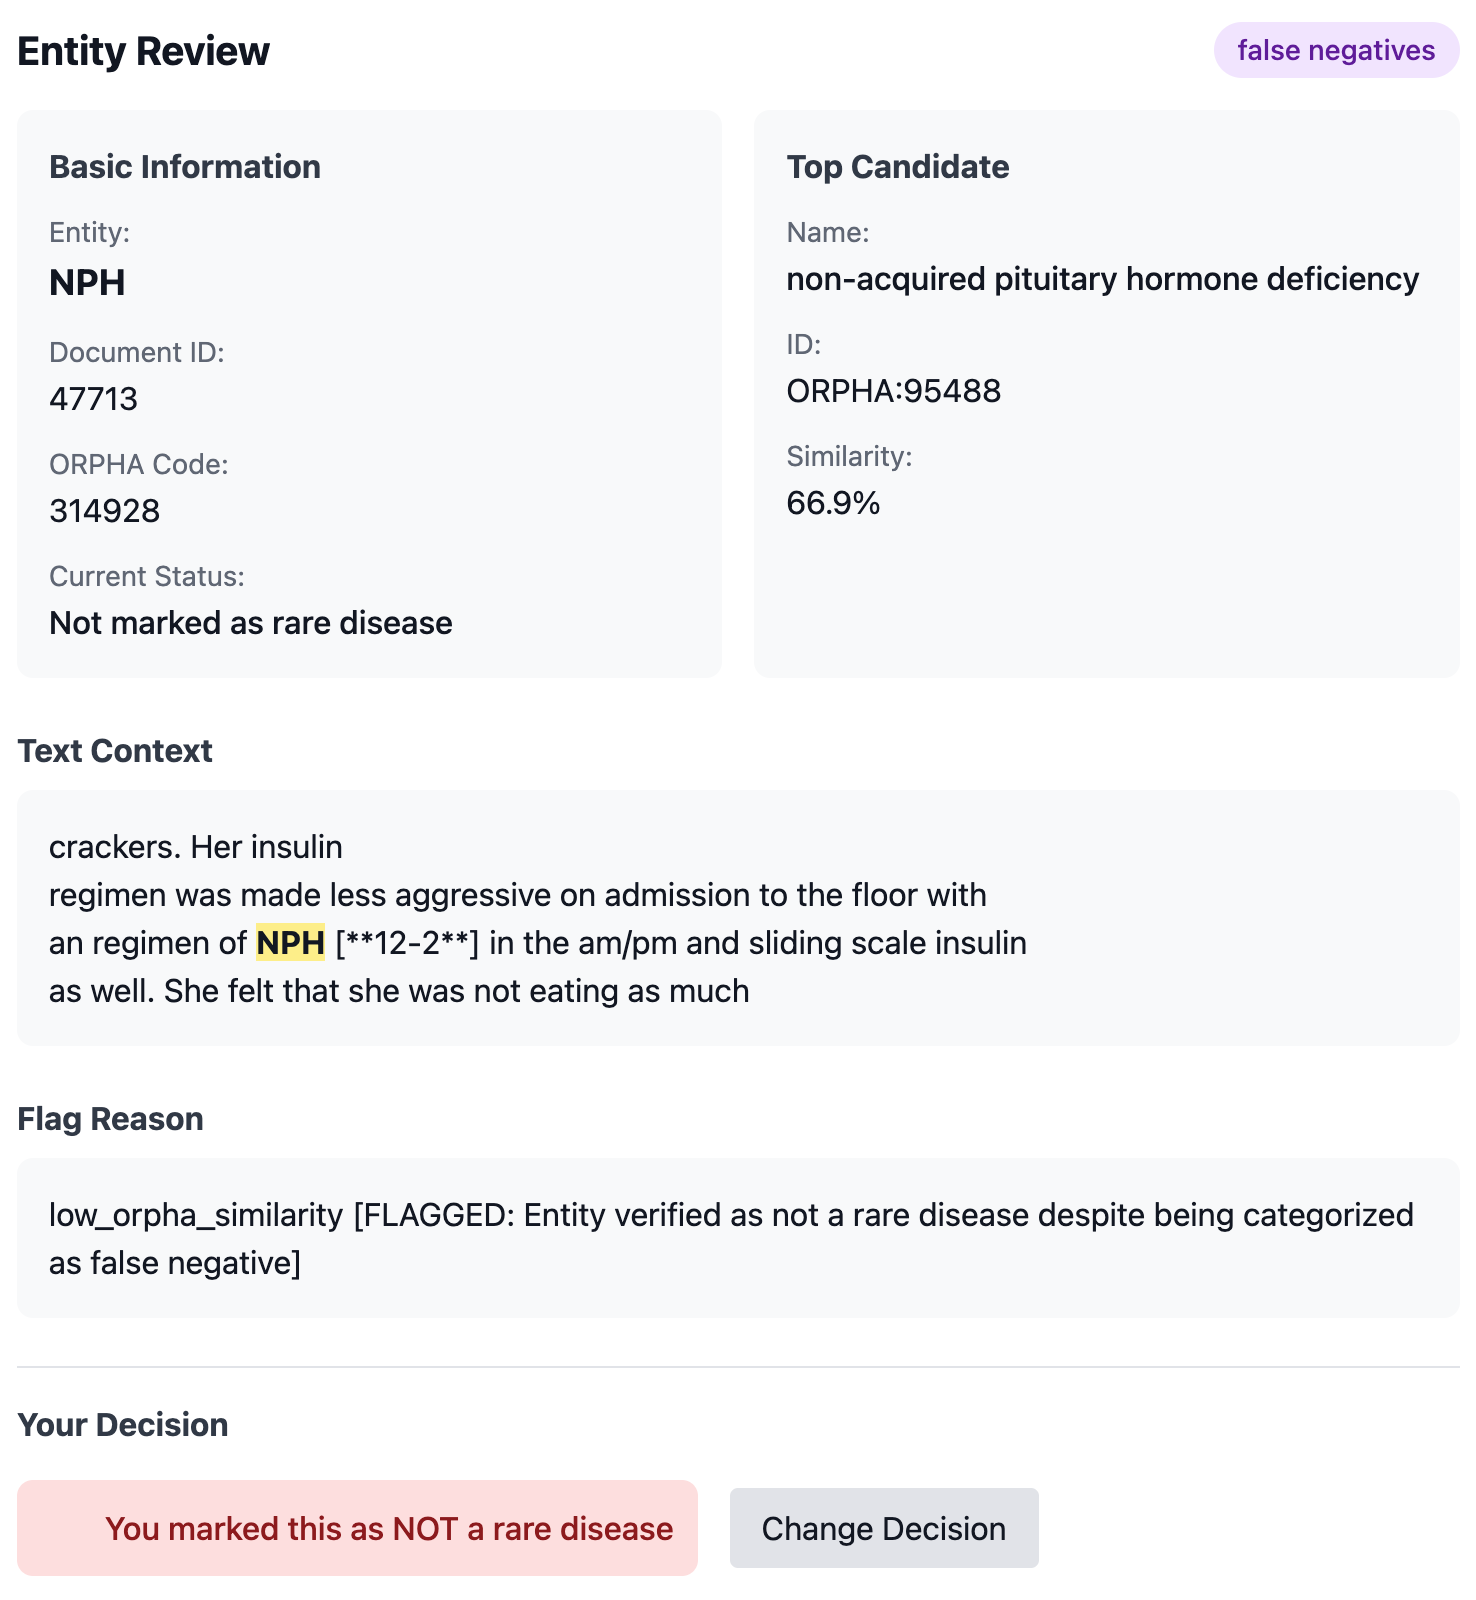
\includegraphics[width=0.55\textwidth]{figs/AnnotationUI.png}
    \caption{\textbf{Example of Inappropriate Annotation in Noisy Dataset.} We note that while NPH as an abbreivation can be related to ``normal pressure hydrocephalus" or other related conditions in the Orphanet ontology as annotated by \cite{dong2023ontology_poor_annotations}, NPH here in this context is actually referring to neutral protamine hagedorn, a type of insulin used to treat diabetes. }
    \label{fig:ex_annotation}
\end{figure}


\begin{figure}[h]
    \centering
    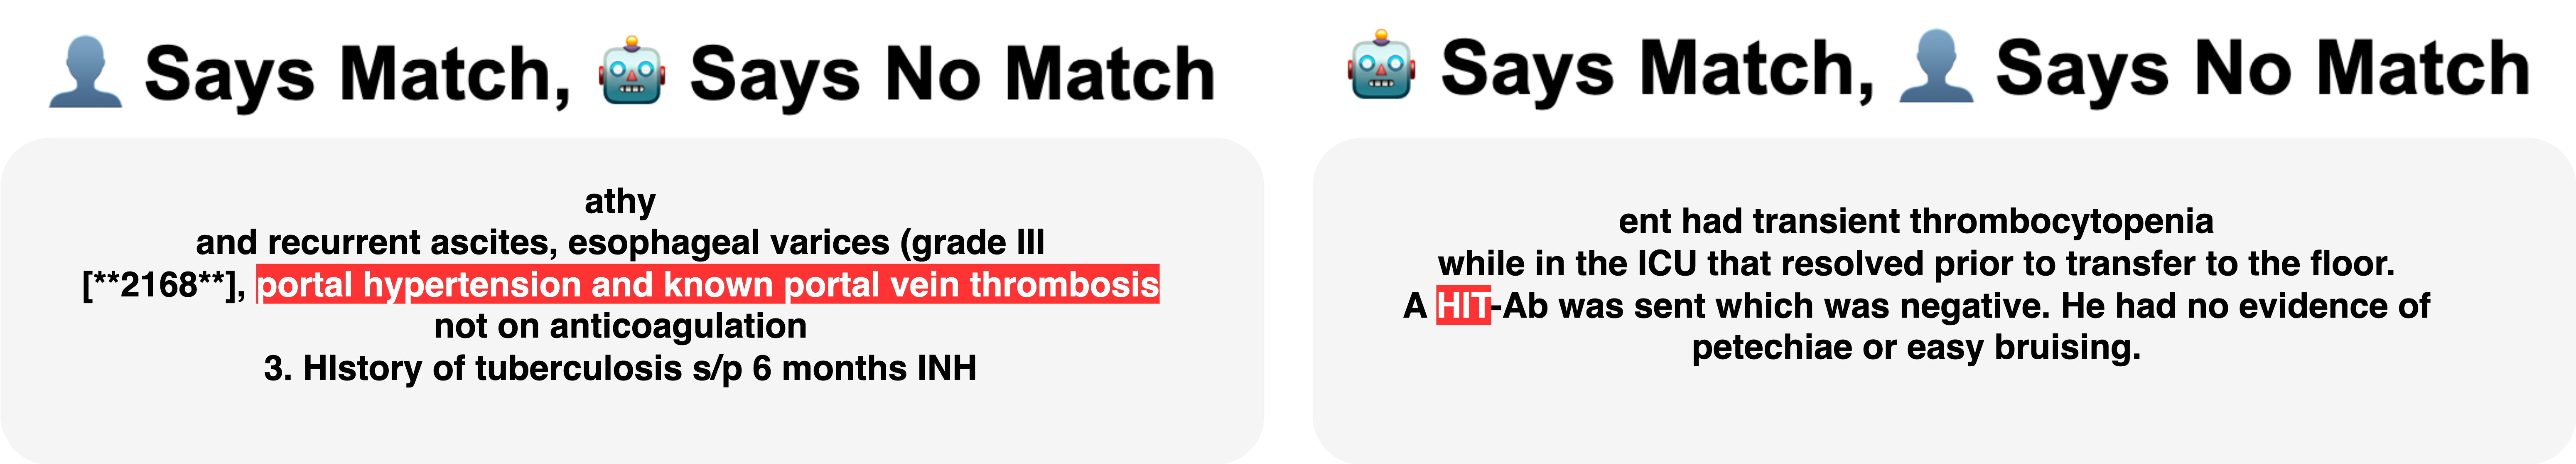
\includegraphics[width=0.8\textwidth]{figs/DisagreementSupervisorVHuman.drawio.png}
    \caption{\textbf{Failure Modes of RDMA in Rare Disease Mining.} When reviewing existing annotations, we showcase two cases where our human annotator disagrees with RDMA's refinement step. Specifically, we see that our refinement agent fails to classify portal vein thrombosis as a rare disease, primarily because its Orphanet listing ``Non-cirrhotic and non-tumoral portal vein thrombosis" does not exactly match the entity ``portal vein thrombosis". On the other hand, while the agent is able to classify ``HIT" as ``heparin induced thrombocytopenia", it does not capture the context "which was negative" properly.}
    \label{fig:annotator_agreement_qualitative}
\end{figure}

\textbf{Examples of RDMA Flagged Entities in Dataset Refinement.} \label{appendix: dataset refinement}
We investigate which entities were primarily flagged by RDMA for human review. We visualize the top cases in Fig. \ref{fig:Top_Corrections}, where we observe that many entities mined by \cite{dong2023ontology_poor_annotations} were indeed not rare diseases, while several key rare disease entities were missed in their original annotations.

\begin{figure}[h!]
    \centering
    \includegraphics[width=1.0\textwidth]{figs/RDMA_Corrections.drawio.png}
    \caption{\textbf{Top 5 Corrected Annotations with RDMA.} RDMA effectively assists human annotation by identifying errors in the noisy historical dataset from \cite{dong2023ontology_poor_annotations}. The figure highlights the top 5 corrections, including both false negatives (a) such as seizure disorder incorrectly labeled as a rare disease in Orphanet, and false positives (b) that were missed in the initial annotations. Of the 72 annotations flagged by RDMA for human review, 55 (76.4\%) were correctly identified as erroneous, demonstrating its value as an annotation assistant for prioritizing human supervision. While hemochromatosis is typically considered a rare condition, in ICU contexts such as MIMIC notes, our physician deemed that to not necessarily be the case. Furthermore, Orphanet \cite{weinreich2008orphanet} makes a distinction between \textbf{rare} hemochromatosis and hemochromatosis. }
    \label{fig:Top_Corrections}
\end{figure}

\clearpage
\section*{Supplementary Note 5: Annotator Guidelines} \label{appendix:annotator guidelines}
\rev{We build on the rare disease mention annotations from \cite{dong2023ontology_poor_annotations} in MIMIC-III, first filtering out clearly erroneous annotations as detailed in Table \ref{tab:Filtering_Details_ex}. Following filtering, a Ph.D. student reviewed each remaining entity from \cite{dong2023ontology_poor_annotations} under physician guidance, applying the review process outlined in Fig. \ref{fig:annotator_guidelines} to determine whether each mention directly or indirectly implies a rare disease. This produced our final curated annotation set.}

\rev{For the RDMA-assisted annotation run, the same Ph.D. student conducted a separate review pass over only the entities flagged by RDMA for human review, applying a binary correction, marking each as correct or incorrect. RDMA flags entities exhibiting disagreement across two independent mining passes and a final agent verification check, meaning the annotator is presented only with the subset of entities where automated agreement could not be established.}

\rev{\paragraph{Inter-Annotator Agreement.} We measure agreement between the human annotator and RDMA using Cohen's $\kappa$, which corrects observed agreement by chance agreement:}
\begin{equation}
    \rev{\kappa = \frac{p_o - p_e}{1 - p_e}}
\end{equation}
\rev{Given a $2 \times 2$ confusion matrix over $N = \text{TP} + \text{TN} + \text{FP} + \text{FN}$ binary judgments, observed agreement and chance agreement are computed as:}
\begin{align}
    \rev{p_o} &\rev{= \frac{\text{TP} + \text{TN}}{N}} \\
    \rev{p_e} &\rev{= p_{\text{human}} \cdot p_{\text{RDMA}} + (1 - p_{\text{human}}) \cdot (1 - p_{\text{RDMA}})}
\end{align}
\rev{where $p_{\text{human}} = (\text{TP} + \text{FN}) / N$ and $p_{\text{RDMA}} = (\text{TP} + \text{FP}) / N$ are the marginal rates of each rater labeling an entity as a rare disease mention. We report $\kappa$ under the Landis \& Koch interpretation bands, where $\kappa \in [0.41, 0.60]$ indicates moderate agreement and $\kappa \in [0.81, 1.00]$ indicates almost perfect agreement. Agreement between the human annotator and the unassisted prior annotations yielded $\kappa = 0.454$ (moderate), while agreement between the human annotator and RDMA-assisted annotations yielded $\kappa = 0.810$ (almost perfect), demonstrating a substantial improvement in annotation quality under the RDMA-assisted workflow.}

\begin{figure}[h!]
    \centering
    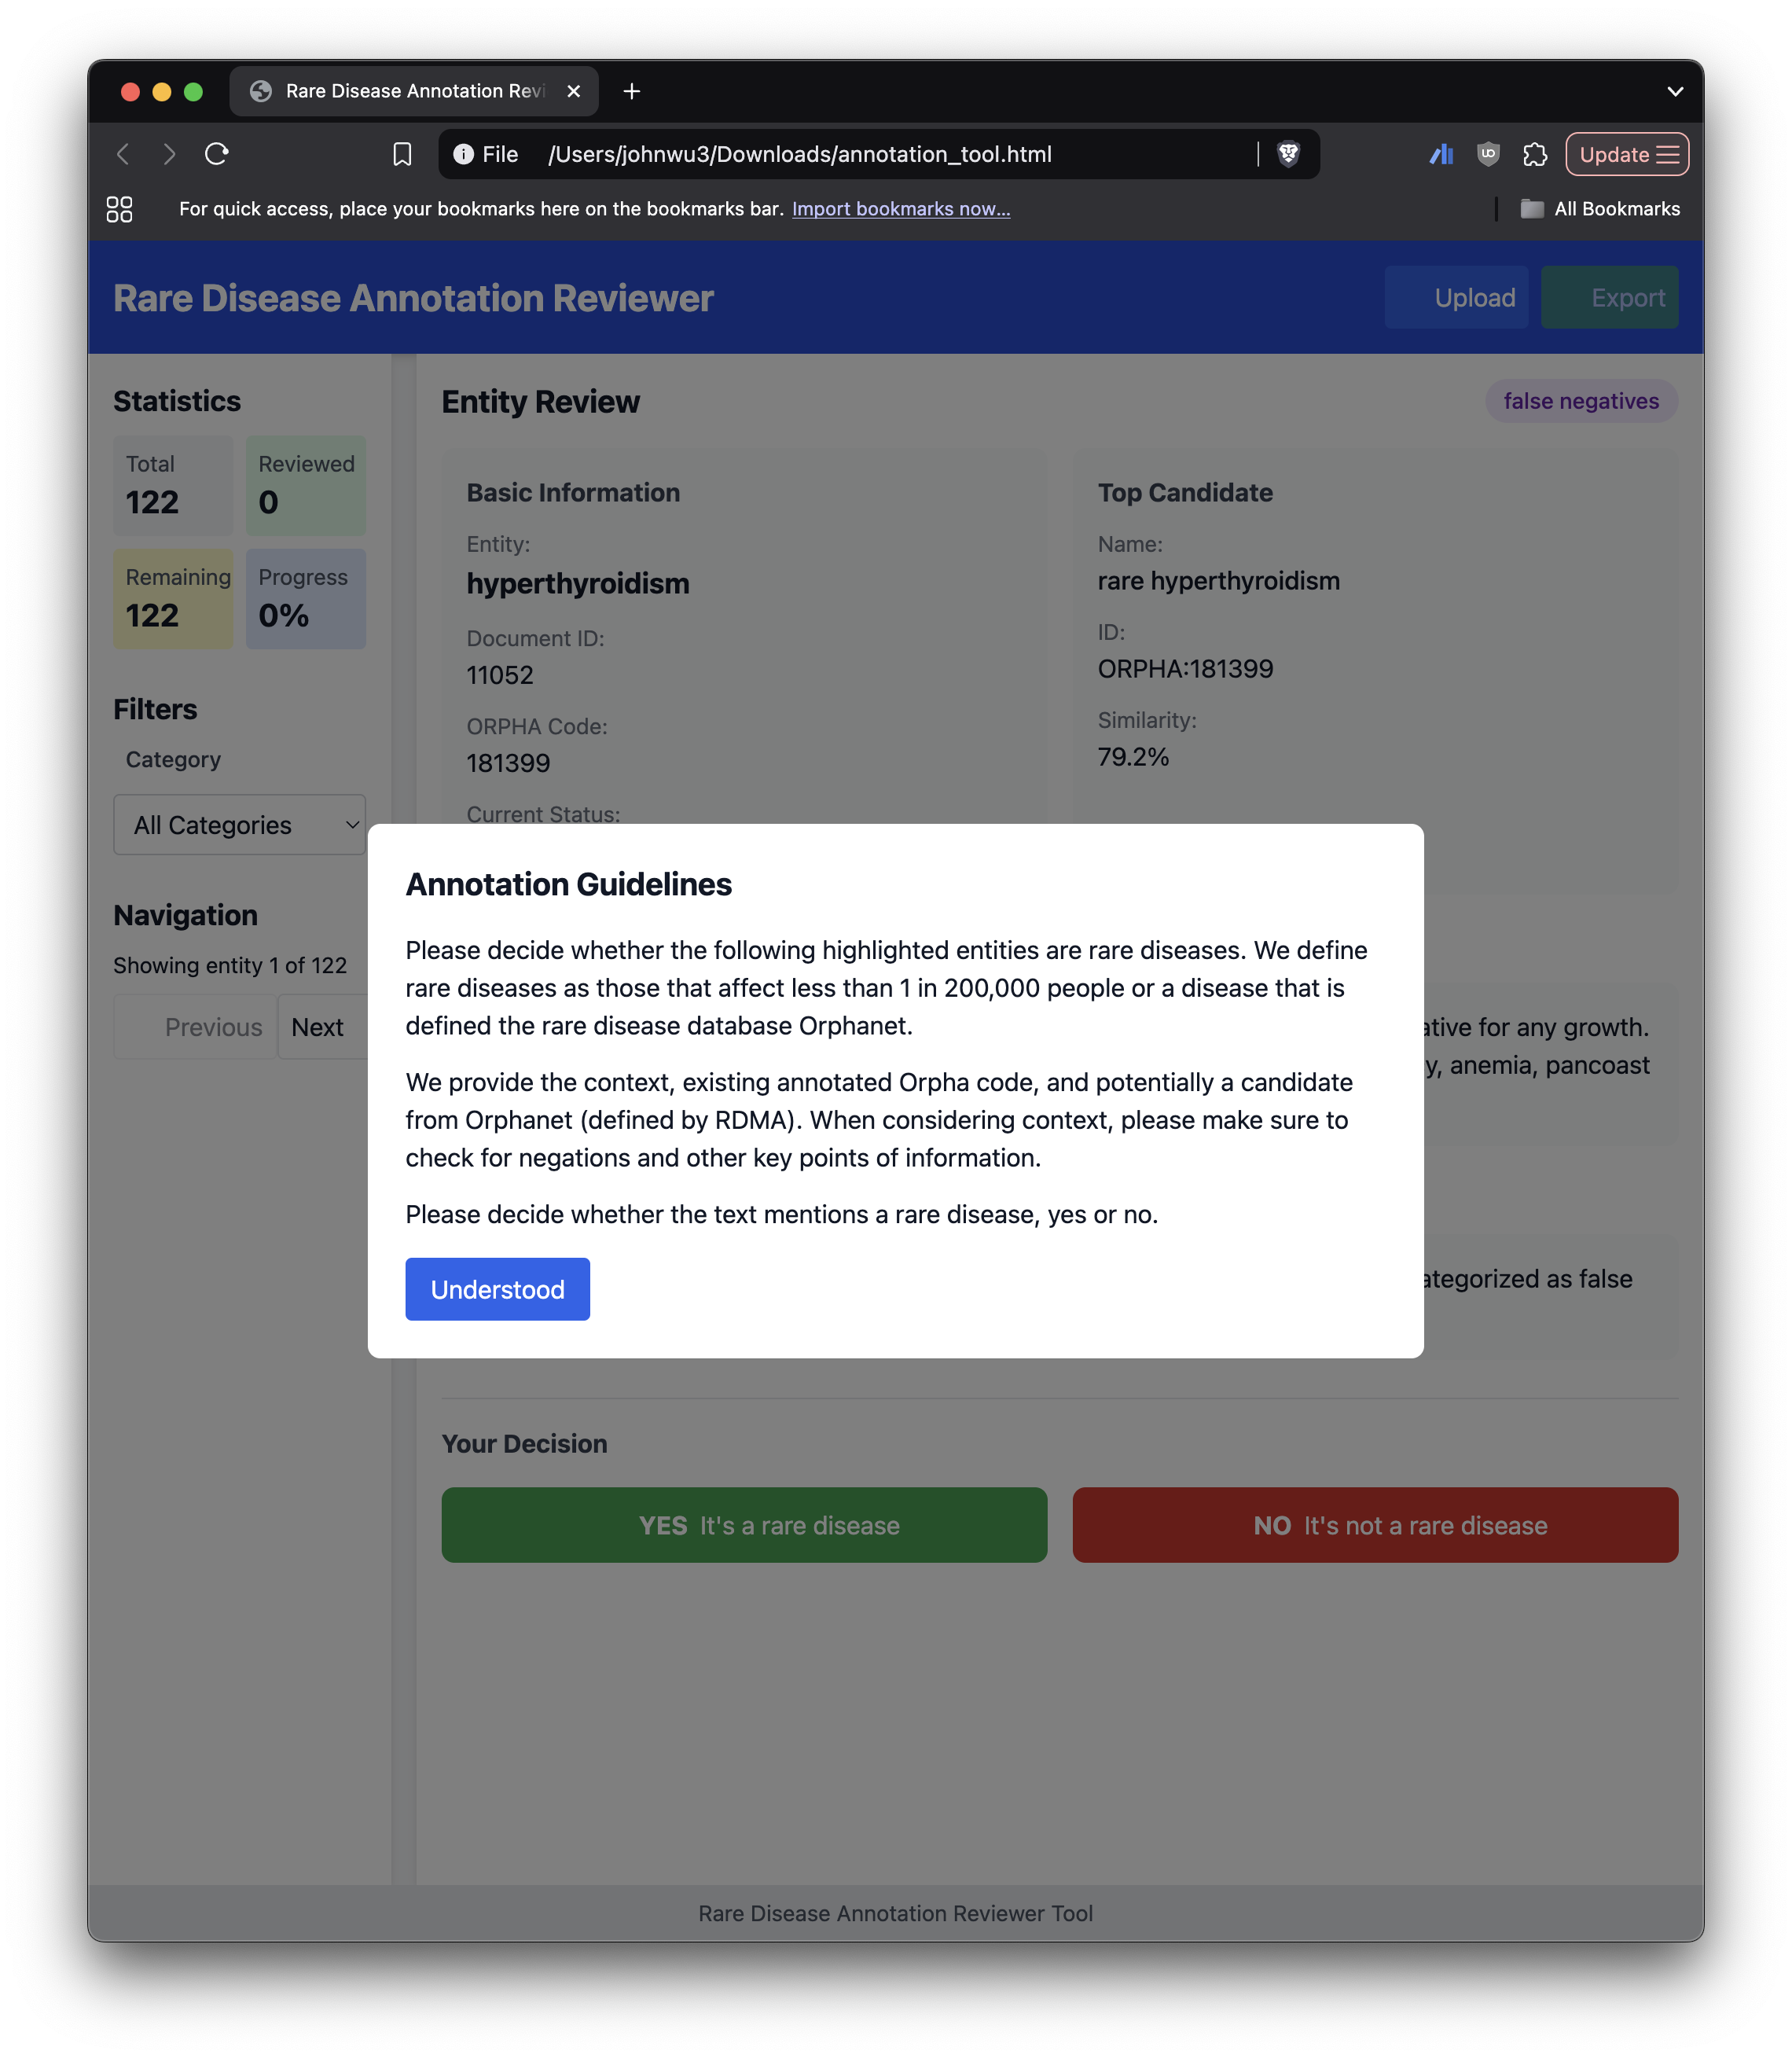
\includegraphics[width=0.8\textwidth]{figs/annotator_guidelines.png}
    \caption{\textbf{Annotator Guidelines.} Annotators are asked if the mention in text directly or indirectly implies a rare disease.}
    \label{fig:annotator_guidelines}
\end{figure}
\supnote{Sentence Agglomeration for Faster Entity Extraction}\label{appendix: sentence agglomeration}

To optimize the performance of our retrieval-enhanced entity extraction process, we implemented a sentence agglomeration strategy that combines shorter sentences to reduce computational costs.

\begin{algorithm}
\caption{Sentence Agglomeration Algorithm}
\begin{algorithmic}[1]
\Procedure{MergeSmallSentences}{$sentences, min\_size$}
    \If{$sentences$ is empty}
        \State \Return empty list
    \EndIf
    \If{$min\_size$ is null or $min\_size \leq 0$}
        \State \Return $sentences$ unmodified
    \EndIf
    
    \State $merged\_sentences \gets$ empty list
    \State $current\_idx \gets 0$
    
    \While{$current\_idx < |sentences|$}
        \State $current\_sentence \gets sentences[current\_idx]$
        
        \If{$|current\_sentence| \geq min\_size$}
            \State Append $current\_sentence$ to $merged\_sentences$
            \State $current\_idx \gets current\_idx + 1$
            \State \textbf{continue}
        \EndIf
        
        \State $merged\_chunk \gets current\_sentence$
        \State $next\_idx \gets current\_idx + 1$
        
        \While{$next\_idx < |sentences|$ \textbf{and} $|merged\_chunk| < min\_size$}
            \If{$merged\_chunk$ is not empty \textbf{and} $sentences[next\_idx]$ is not empty}
                \State $merged\_chunk \gets merged\_chunk + $ " " $+ sentences[next\_idx]$
            \Else
                \State $merged\_chunk \gets merged\_chunk + sentences[next\_idx]$
            \EndIf
            \State $next\_idx \gets next\_idx + 1$
        \EndWhile
        
        \State Append $merged\_chunk$ to $merged\_sentences$
        \State $current\_idx \gets next\_idx$
    \EndWhile
    
    \State \Return $merged\_sentences$
\EndProcedure
\end{algorithmic}
\end{algorithm}


\begin{table}[h]
\centering

\begin{tabular}{l|c|c}
\hline
\textbf{Metric} & \textbf{No Agglomeration} & \textbf{With Agglomeration (Min Size = 500)} \\
\hline
Total documents analyzed & 117 & 117 \\
Average word count per document & 1897 & 1897 \\
Precision & 0.89 & 0.82 \\
Recall & 0.44 & 0.42 \\
F1 score & 0.59 & 0.55 \\
Extraction run time (hours) & 8:36 & 2:09 \\
\hline
\end{tabular}
\caption{\textbf{Comparative Performance Metrics for Different Sized Text Chunks in RDMA for the Entiy Extraction Step.}  We observe that performance declines slightly, but we are able to extract entities at a substantially higher rate (4x faster) from over 200,000 words.}
\end{table}

Sentence agglomeration with a minimum size of 500 characters reduced processing time by 75\% with a modest trade-off in extraction quality, making this approach particularly valuable for time-sensitive applications or large document collections.
\clearpage
\section*{Supplementary Note 7: MIMIC3-RD Preliminary Filtering}
\textbf{Preliminary Filtering.} Before applying our RDMA refinement (Fig. \ref{fig:ex_annotation}), we filter out known incorrect keywords and add known rare disease mentions, as detailed in Table \ref{tab:Filtering_Details_ex}. These changes significantly impact the dataset statistics (Table \ref{tab:filtering_results_ex}), reducing annotations from 1,073 to 333. We use this filtered dataset for our case study in Section \ref{sec: improving existing annotations}.

\begin{table}[h]
\centering
\begin{tabular}{|p{0.3\textwidth}|p{0.7\textwidth}|}
\hline
\textbf{Kept Abbreviations} & HIT, ALS, and NPH \\
\hline
\textbf{Manually Removed Terms} & Hyperlipidemia, dyslipidemia, hypercholesterolemia \\
\hline
\textbf{Manually Added Terms} & papillary carcinoma, glioblastoma multiforme, transitional cell carcinoma, multifocal atrial tachycardia (mat), sarcoidosis, methemoglobinemia, central nervous system and systemic lymphoma, sclerosis cholangitis, mediastinitis, mesenteric vein thrombosis, multiple myeloma, hepatocellular carcinoma, primary cns lymphoma, sclerosing cholangitis, bechet's disease, neovascular glaucoma, meningocele, alopecia, neovascular glaucoma angle closure, pyoderma gangrenosum, budd-chiari, intraductal papillary mucinous tumor, complex tracheal stenosis, cervical stenosis, bronchiectasis, medullary sponge kidney, protein s, antiphospholipid antibody syndrome, protein c, hepatocellular ca, acute myelogenous leukemia, anaplastic thyroid carcinoma, thymoma, congenital bleeding disorder, tracheal stenosis \\
\hline
\end{tabular}
\caption{\textbf{Initial Keyword-based Filtering Attempts} Our clinician identified numerous incorrectly annotated terms from the original entity set. For instance, "MR" was incorrectly tagged as "Multicentric reticulohistiocytosis" in \cite{dong2023ontology_poor_annotations}'s annotations, though it commonly refers to "magnetic resonance". Our clinician flagged all abbreviations except HIT, ALS, and NPH. We also removed common disease terms like hyperlipidemia, as their rare variants are specifically defined differently in the Orphanet ontology. Finally, our clinician manually added the terms listed above. For each added term, we checked its presence in each document and, if found, added an annotation with its corresponding ORPHA code.}
\label{tab:Filtering_Details_ex}
\end{table}

\begin{table}[h]
\centering
\begin{tabular}{l c c}
\hline
\textbf{} & \textbf{Original} & \textbf{After Initial Filtering} \\
\hline
Number of Notes & 312 & 117 \\
Number of Annotations & 1,073 & 333 \\
\hline
\end{tabular}
\caption{\textbf{Rare Disease Annotation Statistics Before and After Initial Keyword Filtering.} We eliminated over 700 misannotated terms before conducting evaluations in Section \ref{sec: improving existing annotations}.}
\label{tab:filtering_results_ex}
\end{table}
\clearpage



\section*{Supplementary Note 9: Prompts}\label{appendix:prompts}
We showcase all of the LLM prompts used in RDMA below.

\begin{figure}[h!]
    \centering
    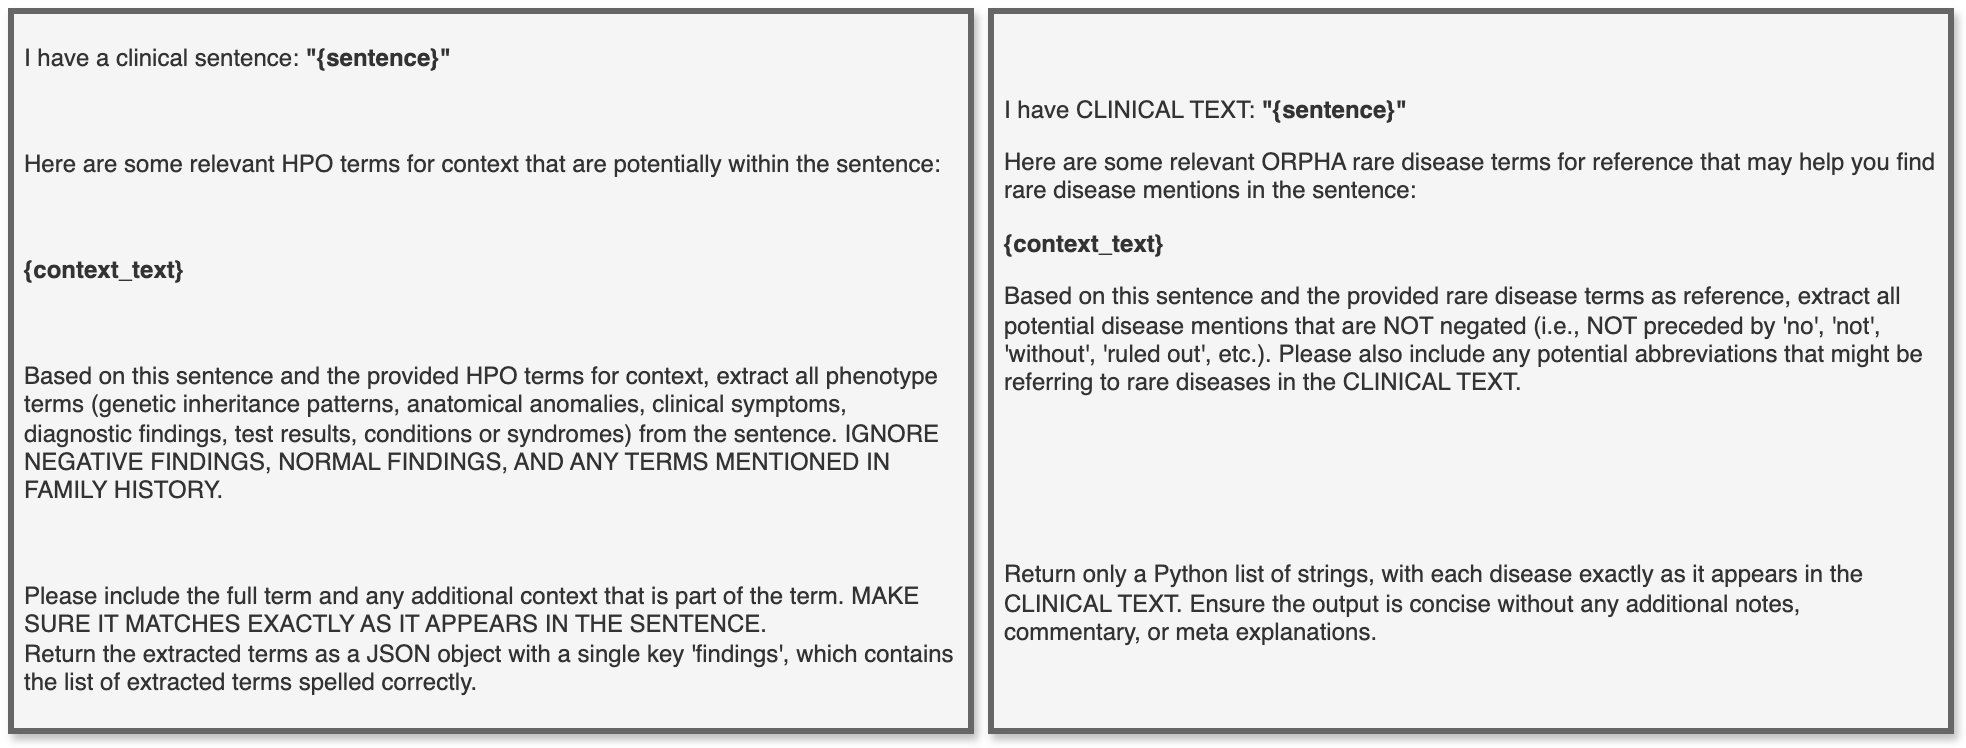
\includegraphics[width=1.0\textwidth]{figs/prompts/RetrievalExtractionPrompt.drawio.png}
    \caption{\textbf{Entity Extraction Prompts.} We showcase both HPO extraction (left) and Rare Disease extraction (right) prompts here.}
    \label{fig:EntityExtractionPrompt}
\end{figure}

\subsection{HPO Verification and Matching Prompts} \label{appendix: HPO prompts}
We showcase all of the prompts used for HPO extraction here. 

\begin{figure}[h!]
    \centering
    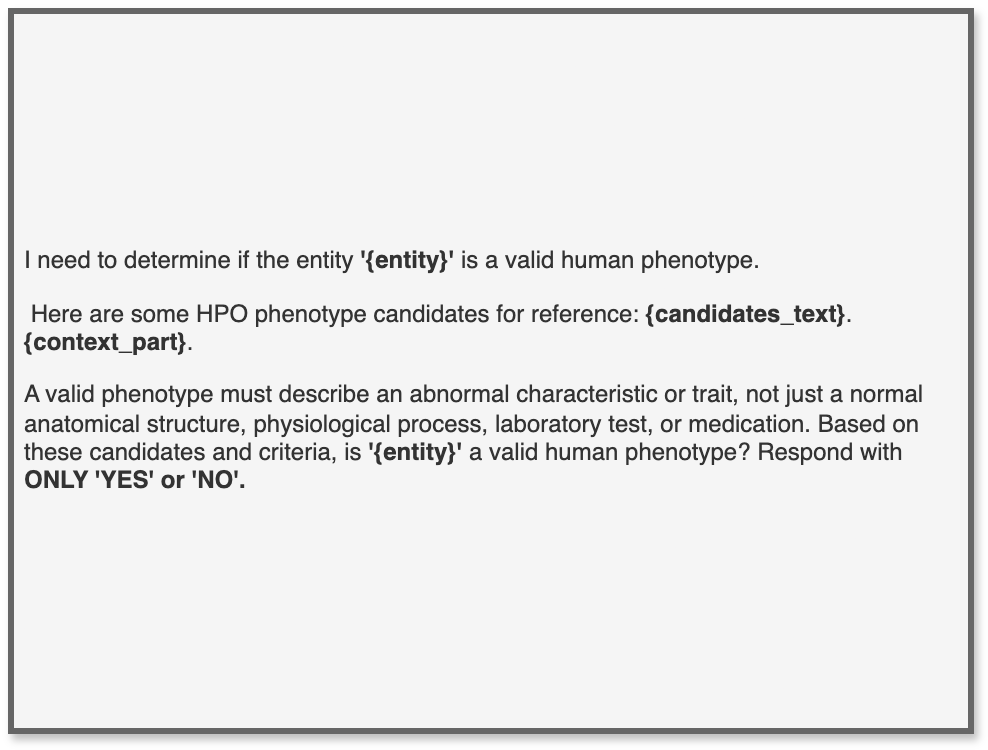
\includegraphics[width=0.8\textwidth]{figs/prompts/hpo/DirectPhenotype.drawio.png}
    \caption{\textbf{Verifying an Entity is a Phenotype.} This reasoning step is used repeatedly in verifying all phenotype implications, whether done by a lab test or a generated implication. }
    \label{fig:DirectPhenotype}
\end{figure}

\begin{figure}[h!]
    \centering
    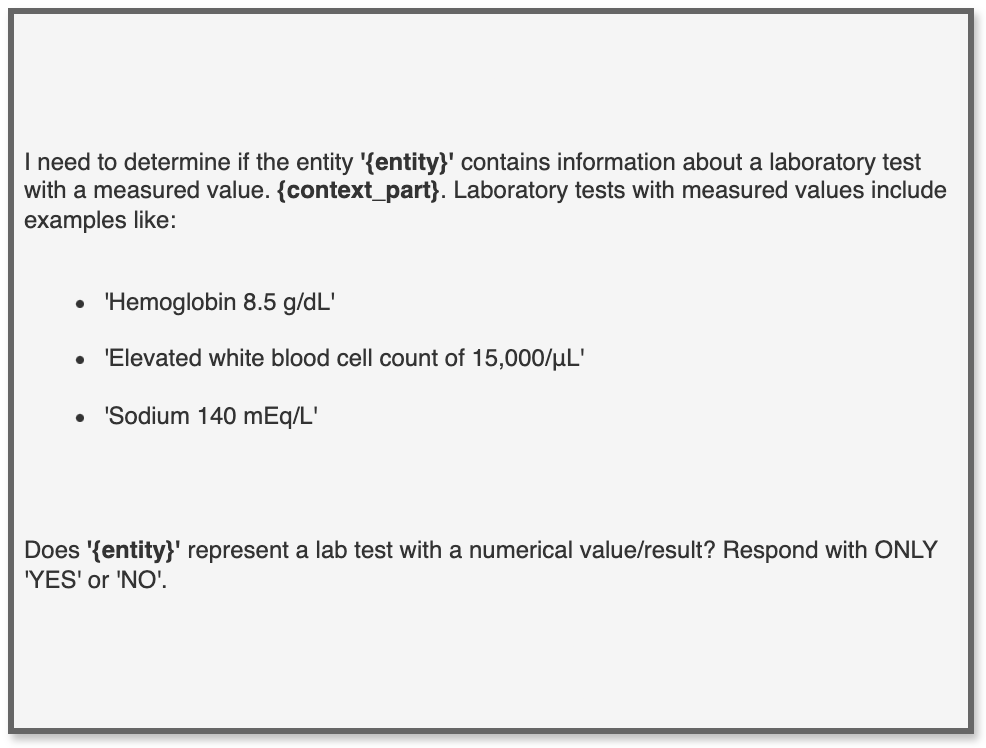
\includegraphics[width=0.8\textwidth]{figs/prompts/hpo/LabTestsCheckPrompt.drawio.png}
    \caption{\textbf{Lab Test Check.} LLMs are asked to see if an entity is indicative of a lab test. }
    \label{fig:LabTestsCheck}
\end{figure}

\begin{figure}[h!]
    \centering
    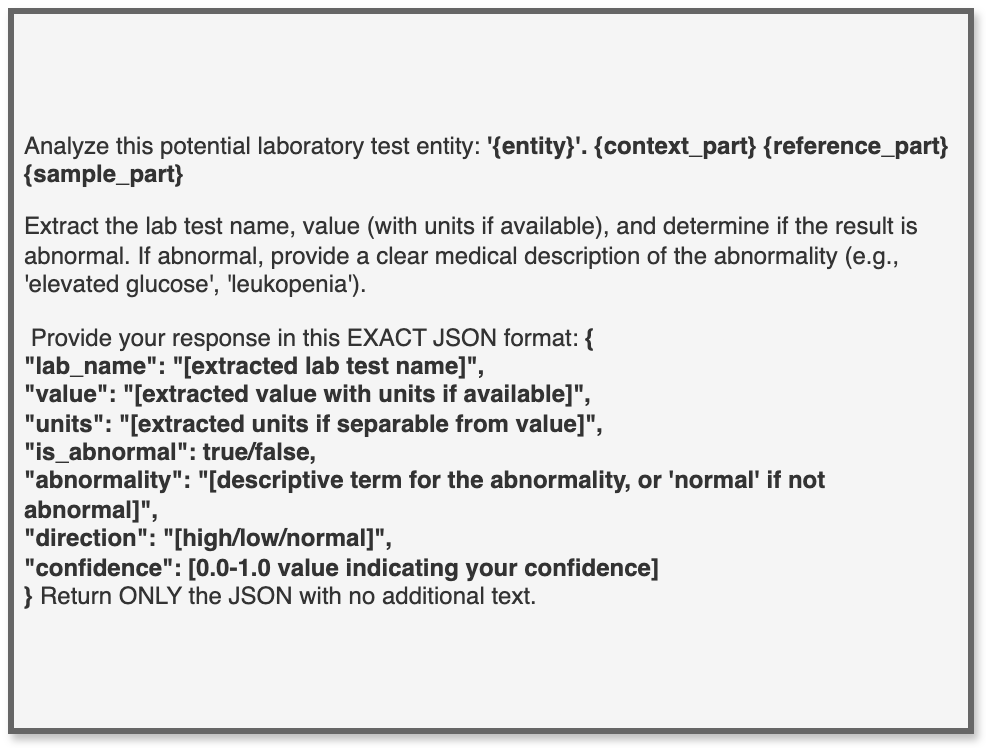
\includegraphics[width=0.8\textwidth]{figs/prompts/hpo/LabTestsAnalysis.drawio.png}
    \caption{\textbf{Lab Test Implication.} LLMs are asked to determine if a lab event indicates an abnormality in the patient.}
    \label{fig:LabTestsAnalysis}
\end{figure}


\begin{figure}[h!]
    \centering
    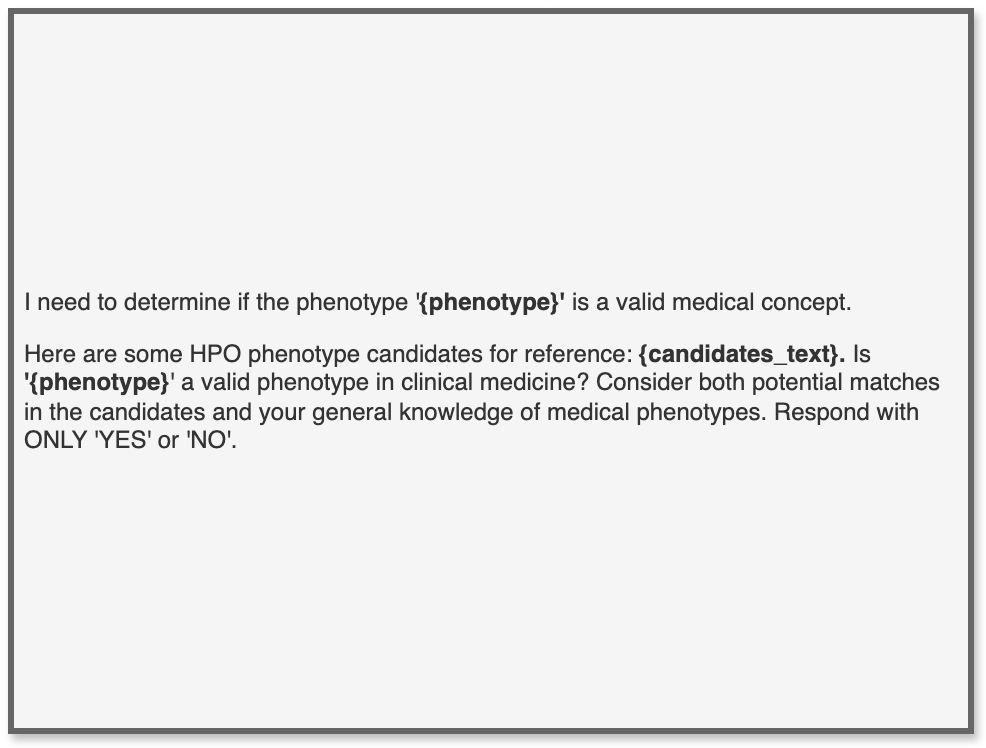
\includegraphics[width=0.8\textwidth]{figs/prompts/hpo/PhenotypeCorrectnessCheck.drawio.png}
    \caption{\textbf{Variant of Phenotype Verification.} This prompt is used to double check if an implied lab test phenotype is within the HPO ontology.}
    \label{fig:PhenotypeCorrectnessCheck}
\end{figure}


\begin{figure}[h!]
    \centering
    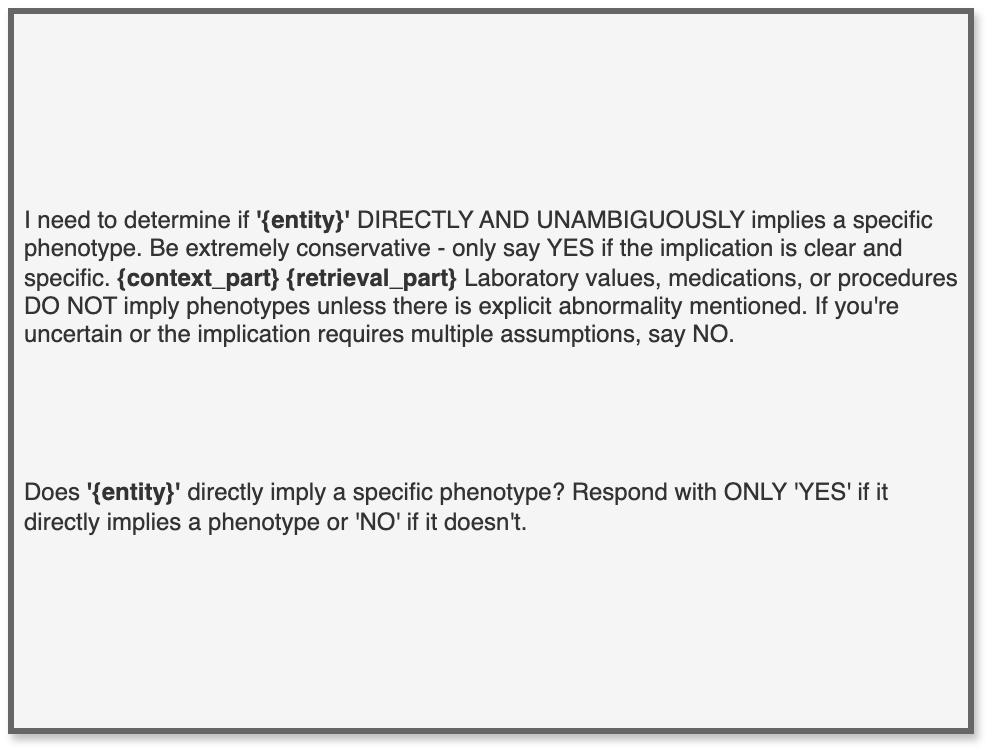
\includegraphics[width=0.8\textwidth]{figs/prompts/hpo/PhenotypeImplicationCheck.drawio.png}
    \caption{\textbf{Entity Implies Phenotype Check.} LLM is asked to check if an entity implies the possibility of a phenotype.}
    \label{fig:CheckIfImpliesPhenotypet}
\end{figure}

\begin{figure}[h!]
    \centering
    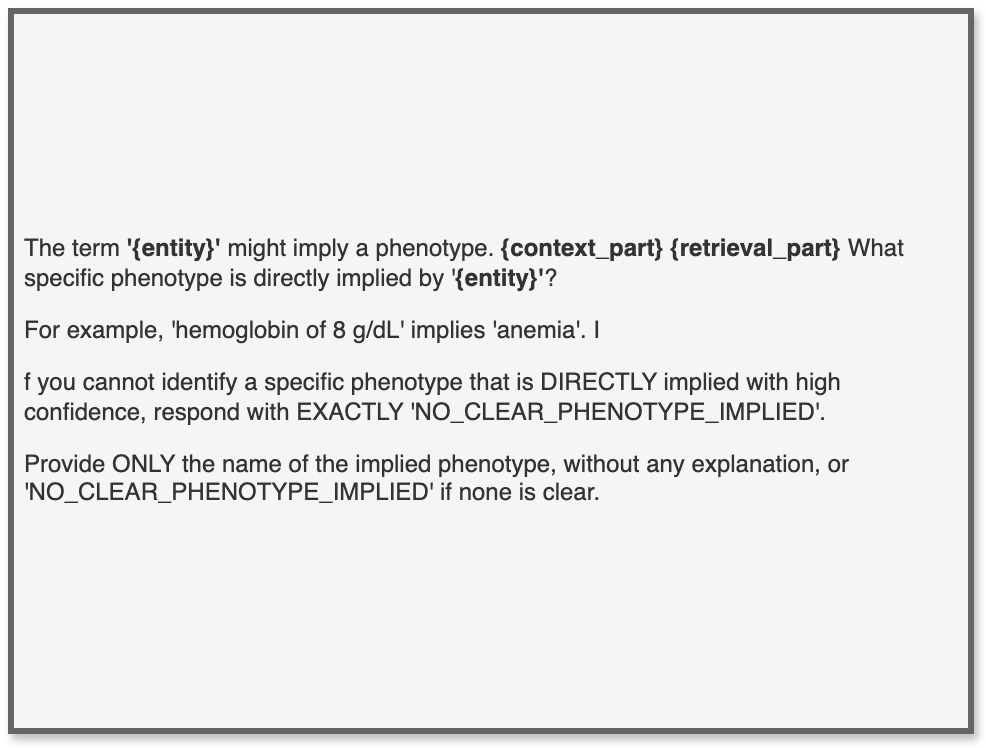
\includegraphics[width=0.8\textwidth]{figs/prompts/hpo/PhenotypeImplicationGeneration.drawio.png}
    \caption{\textbf{Phenotype Implication Generation.} The LLM is asked to generate or predict what the implied phenotype is based on context and the entity.}
    \label{fig:PhenoImplicationGeneration}
\end{figure}

\begin{figure}[h!]
    \centering
    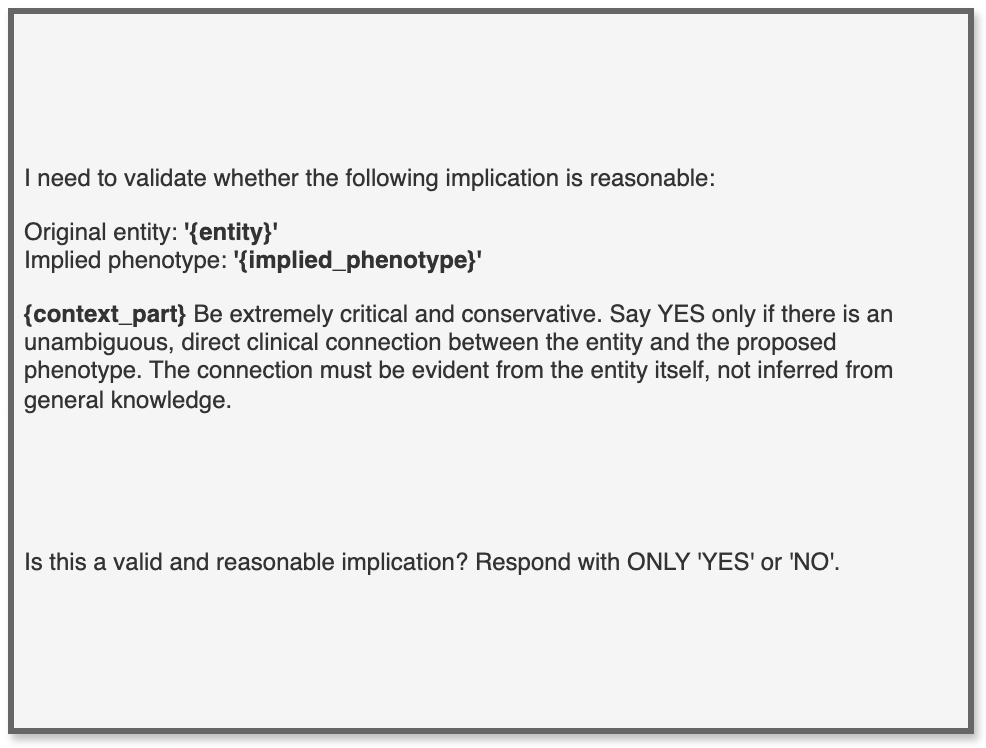
\includegraphics[width=0.8\textwidth]{figs/prompts/hpo/PhenotypeImplicationReasonable.drawio.png}
    \caption{\textbf{Phenotype Implication Reasoning Check.} The LLM is then asked to double check its implication to make sure it makes sense.}
    \label{fig:PhenotypeImplicationReasonableCheck}
\end{figure}

\begin{figure}[h!]
    \centering
    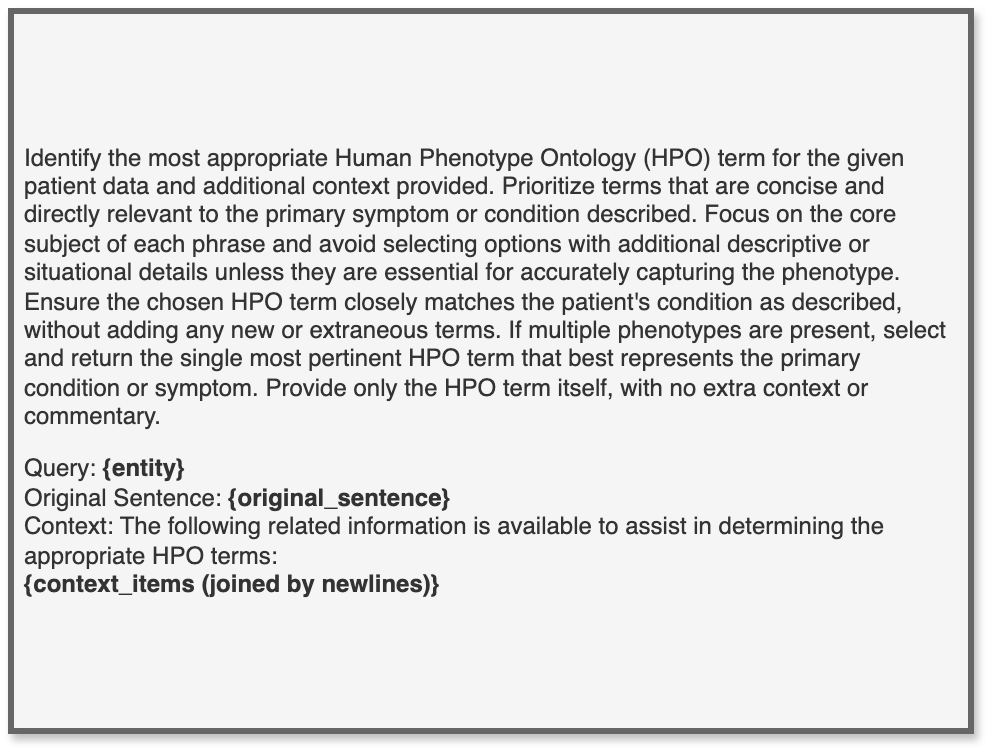
\includegraphics[width=0.8\textwidth]{figs/prompts/hpo/PhenotypeMatching.drawio.png}
    \caption{\textbf{Phenotype Matching.} Finally, the LLM is asked to match the an entity or implied entity to a matching phenotype.}
    \label{fig:PhenotypeMatching}
\end{figure}

\clearpage
\subsection{Rare Disease Verification and Matching Prompts} \label{appendix: rd prompts}

\begin{figure}[h!]
    \centering
    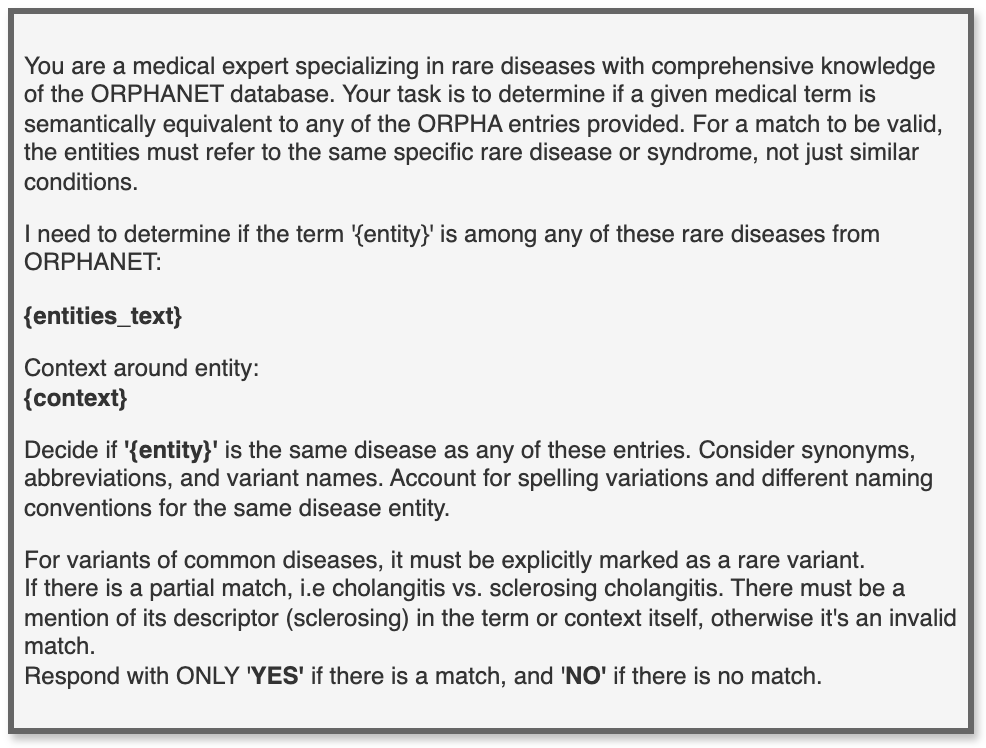
\includegraphics[width=0.8\textwidth]{figs/prompts/rd/RDOntologyCheck.drawio.png}
    \caption{\textbf{Rare Disease Entity Ontology Check.} This prompt checks if the entity is within the Orphanet ontology.}
    \label{fig:RDOntologyCheck}
\end{figure}

\begin{figure}[h!]
    \centering
    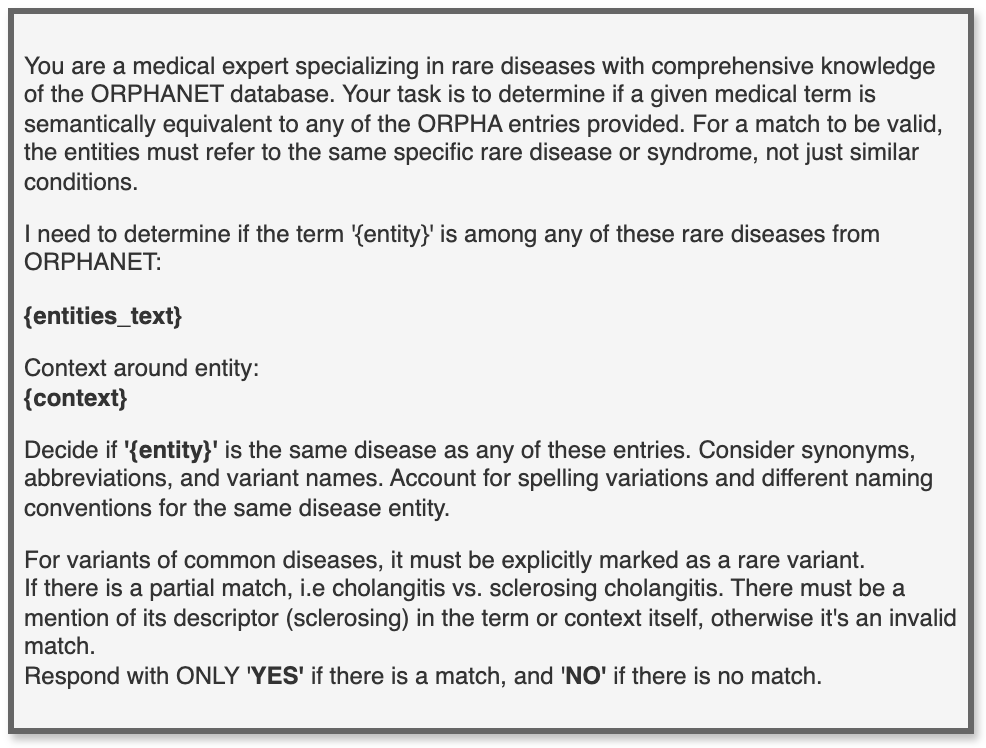
\includegraphics[width=0.8\textwidth]{figs/prompts/rd/RDOntologyCheck.drawio.png}
    \caption{\textbf{Rare Disease Check.} This prompt checks if the entity is actually disease, because not all Orphanet entities are diseases. }
    \label{fig:RDDiseaseCheck}
\end{figure}

\begin{figure}[h!]
    \centering
    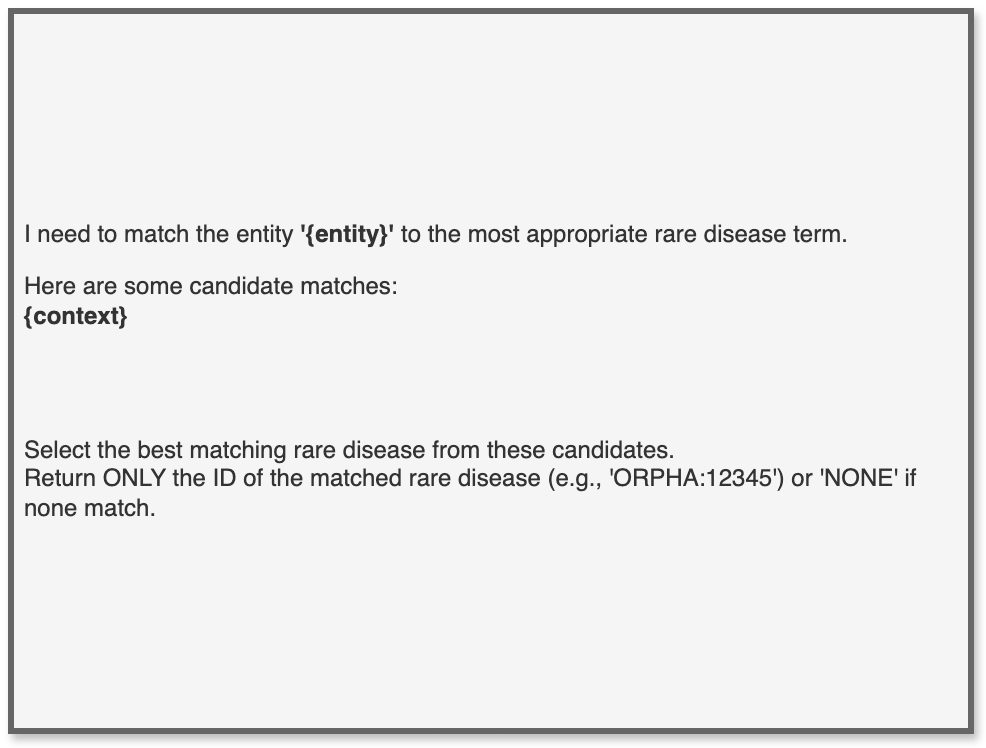
\includegraphics[width=0.8\textwidth]{figs/prompts/rd/RDMatch.drawio.png}
    \caption{\textbf{Rare Disease Matching.} This prompt matches the verified entity to an Orpha code.}
    \label{fig:RDMatch}
\end{figure}


\rev{\subsection{Performance Across Annotation Sets} \label{appendix: rd annotations perf}}
\rev{We disclose what performance metrics look like across the original noisy set of annotations and our different variants of corrected annotations here.}

\begin{table}[h]
\centering
\resizebox{0.8\textwidth}{!}{%
\begin{tabular}{l c c c c}
\hline
\textbf{Baseline} & \textbf{Model} & \textbf{Precision} & \textbf{Recall} & \textbf{F1} \\
\hline
0-shot & Llama 3.3 70B$^q$ & 0.01 & 0.03 & 0.02 \\
Retrieve and String Match & MedEmbed & 0.23 & 0.36 & 0.28 \\
RAG-RD & Mistral 24B$^q$ & 0.17 & 0.45 & 0.24 \\
RDMA & Mistral 24B$^q$ & \textbf{0.67} & \textbf{0.28} & \textbf{0.39} \\
\hline
\multicolumn{5}{c}{\textbf{Human Corrected Labels}} \\
\hline
0-shot & Llama 3.3 70B$^q$ & 0.01 & 0.05 & 0.02 \\
Retrieve and String Match & MedEmbed &  0.25 & 0.43 & 0.32 \\
RAG-RD & Mistral 24B$^q$ & 0.14 & \textbf{0.54} & 0.22 \\
RDMA & Mistral 24B$^q$ & \textbf{0.66} & 0.38 & \textbf{0.48} \\
\hline
\end{tabular}%
}
\caption{\textbf{Rare Disease Extraction Performance Comparison.} We showcase performance on the other 2 sets of rare disease mention labels, the noisy original and the human only corrected labels. We observe that RDMA has significantly higher precision than its baselines, and that it overall outperforms all of its baselines in F1. \textbf{Bold} denotes best performance.}
\label{tab:label_correction}
\end{table}


\end{document}
